
\section {Online Monitoring}

The SVT will be monitored online using the Java based HPS Monitoring Application.
The most basic set of plots can be brought up by issuing the following commands 
from a terminal:  

\begin {itemize}
    \item Log into any PC in the counting house as \texttt{hpsrun}
    \item Issue the command \texttt{startSVTHitPlots} to open the monitoring app
\end {itemize}
Pressing the connect button will bring up plots of SVT occupancies, raw hit counts
and raw hit ADC sample amplitudes. Pressing it again will disconnect the monitoring app and reset all plots.

The command \texttt{startSVTHitPlots -h} will print a list of additional options.

\subsection {Occupancies}

Occupancy in each sensor should rise smoothly from 0 to a peak occupancy between 0.0005 to 0.01. If it doesn't:
\begin{enumerate}
\item Check that SVT bias is on (measured voltage at 180 V for every sensor). If not, bring bias up (reset beam interlock if necessary, then push the "180V" button on the bias GUI) and reset the plots.
\item If occupancies still look bad, start a new run. Reset the plots.
\item If occupancies still look bad, post plot to logbook with the run number, and page expert.
\end{enumerate}

\begin{figure}[ht!]
    \centering
    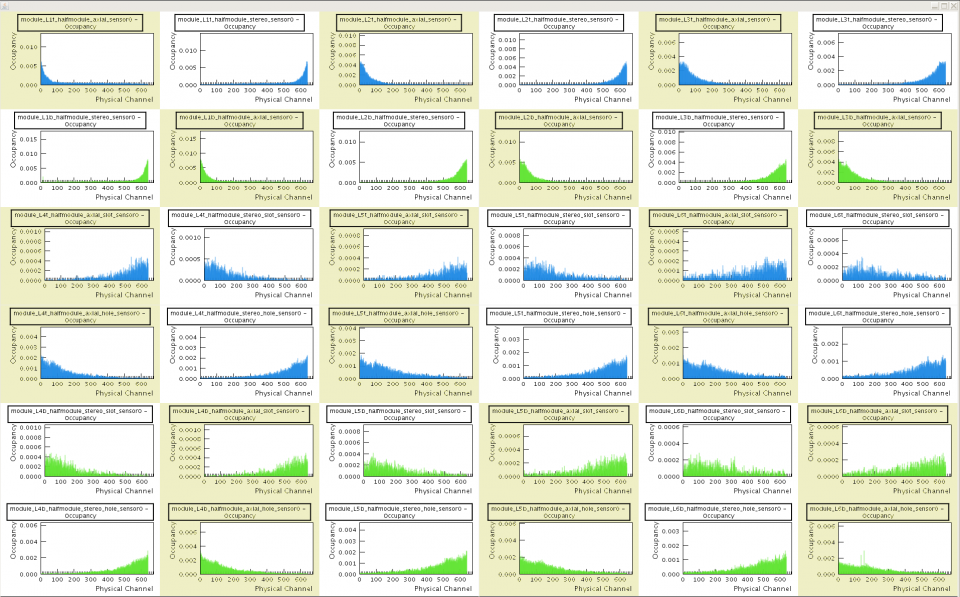
\includegraphics[width=\textwidth]{figures/occupancy_good}
    \caption{SVT occupancies plot.}
    \label{fig:occupancies}
\end{figure}

\begin{figure}[ht!]
    \centering
    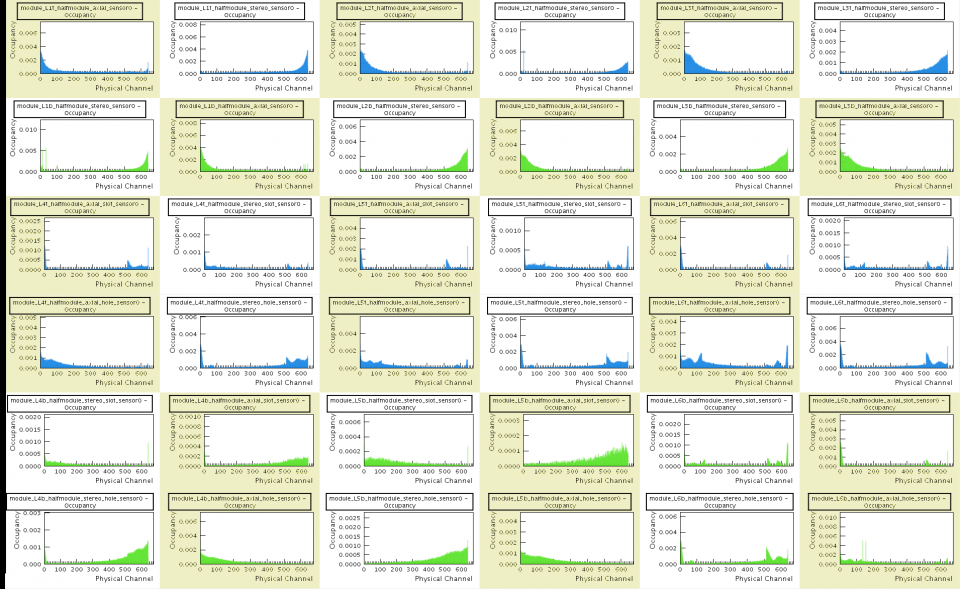
\includegraphics[width=\textwidth]{figures/occupancy_nobias}
    \caption{SVT occupancies plot. Bumpy patterns on many sensors indicate the bias is off or set to 5 V by the beam interlock. Reset the beam interlock, and reset the monitoring app after bias is restored.}
    \label{fig:occupancies_nobias}
\end{figure}

\begin{figure}[ht!]
    \centering
    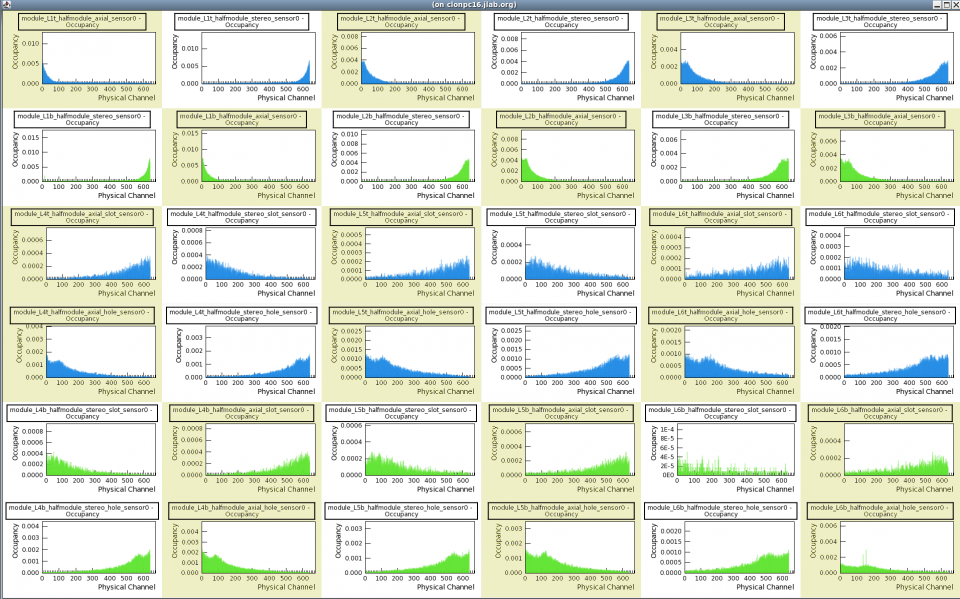
\includegraphics[width=\textwidth]{figures/occupancy_badhybrid}
    \caption{SVT occupancies plot. One sensor (second from bottom, second from right) has low occupancy. Log the plot and start a new run.}
    \label{fig:occupancies_badhybrid}
\end{figure}

\subsection {Samples}
The SVT readout should be in time with the trigger, so that hits from a triggered event show up at a consistent time. The SVT reads out six samples for each trigger; in-time hits should consistently have sample 3 (zero-indexed) be the high sample. This is checked in the max sample plot.

\begin{figure}[ht!]
    \centering
    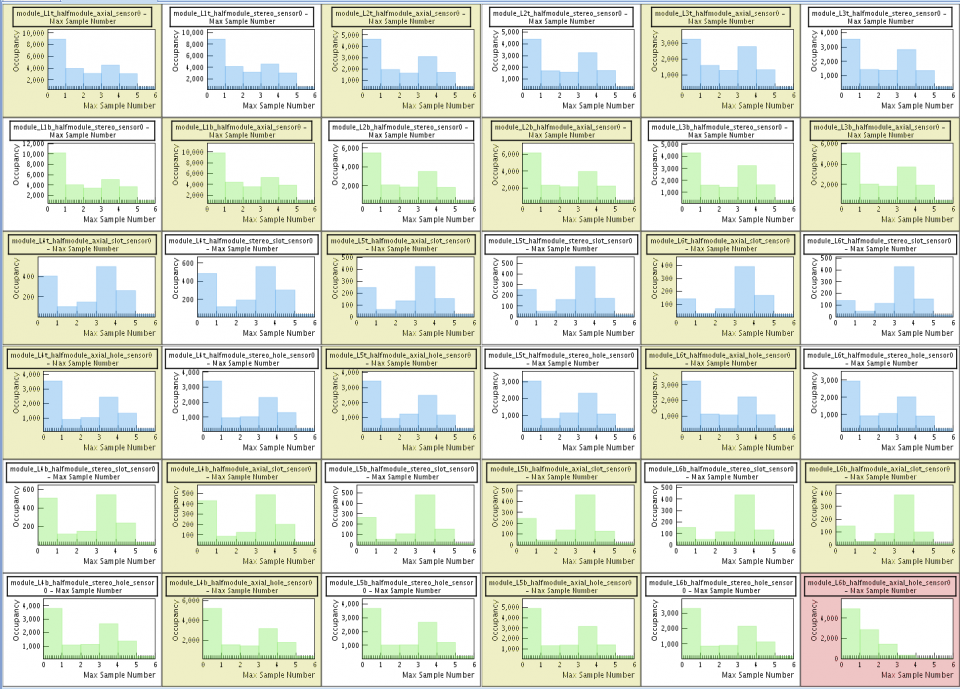
\includegraphics[width=\textwidth]{figures/maxsample_badhybrid}
    \caption{SVT occupancies plot. One sensor (bottom right) is out of time. Log the plot and start a new run.}
    \label{fig:maxsample_badhybrid}
\end{figure}


